\chapter{SonarQube}
\label{chap:sonar}

\section{Sobre o SonarQube}

O Sonar é uma plataforma para gerenciamento de qualidade de código. Esta ferramenta abrange 7 eixos de qualidade de código: Arquitetura e Design, duplicidade, testes unitários, complexidade, erros em potencial, regras de codificação e comentários.

\begin{figure}[h!]
\centering
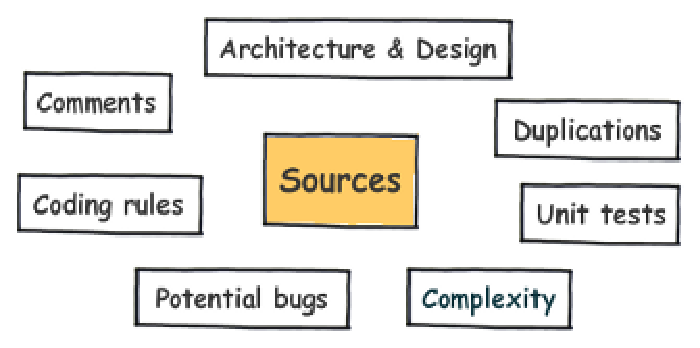
\includegraphics[keepaspectratio=false,scale=0.90]{figuras/figuras_nilton/eixosqualidade.eps}
\caption{7 eixos da qualidade de software 
\citeonline{SonarQube}}
\label{7eixosqualidade}
\end{figure}
%---------------------------------------------------------------------------------------------------------------------%